\documentclass{article}
\setlength{\parskip}{0pt} % esp. entre parrafos
\setlength{\parindent}{3pt} % esp. al inicio de un parrafo
\usepackage{amsmath} % mates
\usepackage{listings}
\usepackage[sort&compress,numbers]{natbib} % referencias
\usepackage{url} % que las URLs se vean lindos
\usepackage[top=10mm,left=20mm,right=20mm,bottom=25mm]{geometry} % \textbf{\textbf{}}margenes
\usepackage{hyperref} % ligas de URLs
\usepackage{graphicx} % poner figuras
\usepackage[spanish]{babel} % otros idiomas
\hypersetup{
    colorlinks=true,
    linkcolor=blue,
    filecolor=blue,      
    urlcolor=blue,
    citecolor=black,
}

\title{TAREA \# 5 \\ Método Monte-Carlo} %titulo
\author{Natalia Berenice P\'{e}rez L\'{o}pez} % author
\date{\today}

\begin{document} % inicia contenido

\maketitle % cabecera

\section{Objetivo}
El objetivo de esta práctica es estudiar estadísticamente la convergencia de la precisión del estimado de la integral con en método Monte-Carlo, comparado con el valor producido por \texttt{Wolfram Alpha}, en términos del número de decimales correctos, aumentando el tamaño de muestra.

\section{Desarrollo} % seccion y etiqueta
Para generar el código objetivo de esta práctica primero se realizó un código que solamente compara los decimales de dos números y muestra como resultado la cantidad de decimales que coinciden entre ellos, para esto se realizaron algunas ideas de código, las cuales se encuentran en \href{https://github.com/nataliaperez0/Simulation/tree/main/Tarea5}{mi repositorio}  en GitHub. A continuación se muestra el código generado: 

\definecolor{verde}{rgb}{0,0.56,0.22}
\definecolor{codegray}{rgb}{0.5,0.5,0.5}
\definecolor{codegreen}{rgb}{0,0.56,0.22}
\definecolor{backcolour}{rgb}{0.95,0.95,0.92}
\definecolor{azul}{rgb}{0,0,1}

\lstdefinestyle{mystyle}{
    backgroundcolor=\color{backcolour},   
    commentstyle=\color{verde},
    keywordstyle=\color{azul},
    numberstyle=\tiny\color{codegray},
    stringstyle=\color{codegreen},
    basicstyle=\ttfamily\footnotesize,
    breakatwhitespace=false,         
    breaklines=true,                 
    captionpos=b,                    
    keepspaces=true,                 
    numbers=left,                    
    numbersep=5pt,                  
    showspaces=false,                
    showstringspaces=false,
    showtabs=false,                  
    tabsize=2
}

\lstset{style=mystyle}
\begin{lstlisting}[language=R, caption= Código para obtener la cantidad de decimales que coinciden entre dos números.]
#IDEA 4
bueno = 0.048834 #numero de Wolfram Alpha
prueba = 0.048214

n = seq(1, 6, 1)

for (i in n) {
  b = trunc(bueno*10^i)/10^i
  p = trunc(prueba*10^i)/10^i
  
  if (p == b) {
    deci = i
  } else {
    print(deci)
    break
  }
}
\end{lstlisting}

Posteriormente, se utilizó como base el código revisado en clase \citep{1} para calcular el valor de la integral definida \eqref{integral} para la función \eqref{funcion} utilizando el método Monte-Carlo.

\begin{equation} 
 \int_{3}^{7} f(x) dx 
\label{integral}
\
\end{equation}

\begin{equation}
f(x) = \frac{1}{exp(x) + exp(-x)}
\label{funcion}
\end{equation}
\smallskip

Este código permite generar números pseudoaleatorios con la distribución de la función \eqref{ecuacion3}, para así estimar la integral definida \eqref{integral2} y después normalizar el estimado para que sea la integral definida \eqref{integral}.

\begin{equation}
g(x) = \frac{2 f(x)}{\pi}
\label{ecuacion3}
\end{equation}

\begin{equation} 
 \int_{3}^{7} g(x) dx 
\label{integral2}
\
\end{equation}
\smallskip

Utilizar la función \eqref{ecuacion3} es posible porque es una función de distribución válida, ya que su integral es igual a 1 \eqref{integral3}.

\begin{equation} 
 \int_{-\infty}^{\infty}\frac{2}{\pi} f(x) \text{d}x = 1
\label{integral3}
\
\end{equation}

Las modificaciones que se le realizaron al código revisado en clase \citep{1} fueron; agregar un ciclo \texttt{for} para variar la \texttt{muestra} en tamaños de $1000$, $10000$, $100000$, $1000000$ y $10000000$, agregar otro ciclo \texttt{for} para hacer $30$ réplicas con cada tamaño de \texttt{muestra} y agregar el código mostrado anteriormente para obtener la cantidad de decimales que coninciden entre el valor de la integral definida \eqref{integral} calculado con el método Monte Carlo y el valor que se obtiene con el programa \texttt{Wolfram Alpha} para dicha integral, el cual es de $0.048834$. A continuación se muestra el código modificado para esta práctica:

\lstset{style=mystyle}
\begin{lstlisting}[language=R, caption= Código para obtener la cantidad de decimales que coinciden al comparar el valor de la integral \eqref{integral} calculado con el método Monte Carlo y el valor que se obtiene con el programa \texttt{Wolfram Alpha}.]
library(ggplot2)
desde = 3
hasta = 7
bueno = 0.048834 #numero de Wolfram Alpha
n = seq(1, 6, 1)
muestra = c(10^3, 10^4, 10^5, 10^6, 10^7) # puntitos en el cuadro
df = data.frame()

for (m in muestra){
  for (replica in 1:30){
    f <- function(x) { return(1 / (exp(x) + exp(-x))) } # funcion que piden
    g <- function(x) { return((2 / pi) * f(x)) } # normalizado a distr
    
    suppressMessages(library(distr)) # paquete
    generador  <- r(AbscontDistribution(d = g)) # creamos un generador
    valores <- generador(m) # generamos valores
    montecarlo = sum(valores >= desde & valores <= hasta) # checamos
    integral <- sum(montecarlo) / m # tasa: integral para g(x)
    resultado <- (pi / 2) * integral # integral para f(x) (renorm)
    for (i in n) {
      b = trunc(bueno*10^i)/10^i
      r = trunc(resultado*10^i)/10^i
      
      if (r == b) {
        deci = i
      } else {
        break
      }
    }
    datos <- c(m, replica, resultado, deci)
    df = rbind(df, datos)
    #cat(m, replica, resultado, deci,'\n')
  }
}

names(df) <- c("Muestra", "Replica", "Resultado", "Decimales")
df$Muestra = as.factor(df$Muestra)
ggplot(df, aes(x= Muestra, y= Decimales, fill= Muestra)) + 
  geom_boxplot()+
  labs(x = "Muestra", y = "Decimales correctos") + #nombres
  scale_x_discrete(labels = c("1K", "10K", "100K", "1M", "10M"))+
  scale_fill_discrete(labels = c("10^3", "10^4", "10^5", "10^6", "10^7"))
\end{lstlisting}

Para analizar los resultados obtenidos se graficaron en un diagrama caja-bigote (Ver figura \ref{Figura1}). En este diagrama podemos ver que al aumentar el tamaño de la muestra se obtiene como resultado un valor más preciso, es decir el valor de la integral con el método Monte Carlo es más parecido al resultado generado con el programa \texttt{Wolfram Alpha.} Por lo tanto se podría decir que a mayor tamaño de muestra, mayor es la precisión de decimales. 
\bigskip

Para analizar si existe una relación entre la variación del tamaño de muestra y la cantidad de decimales correctos, primero se elegió utilizar la prueba estadística ANOVA de una vía, pero debido a los resultados obtenidos al revisar la normalidad de los datos, se eligió realizar la prueba estadística \texttt{Kruskal Wallis} \citep{2}.
\bigskip


\newpage
.
\bigskip

\begin{figure} [h!]% figura
    \centering
    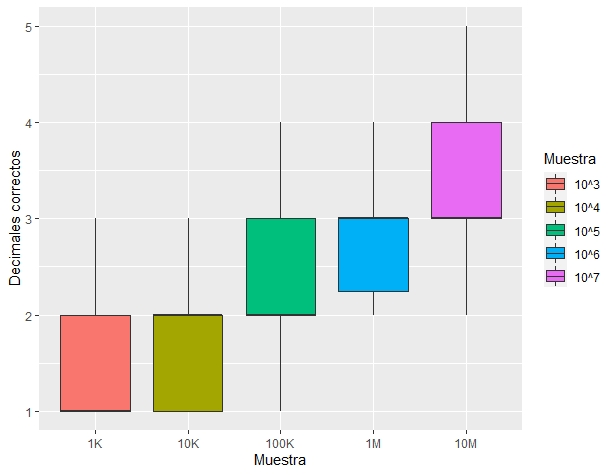
\includegraphics[width=150mm]{Figura1.jpeg} % archivo
    \caption{Cantidad de decimales que coinciden al variar el tamaño de la muestra en la comparación del valor de la integral \eqref{integral} calculado con el método Monte Carlo y el valor que se obtiene del programa \texttt{Wolfram Alpha.}}
    \label{Figura1}
\end{figure}

En el cuadro \ref{Cuadro1} se  resumen los resultados de la revisión de los supuestos para poder aplicar la prueba estadística ANOVA. El supuesto outliers se refiere a la cantidad de valores atípicos que existen en los grupos, la normalidad por grupos se obtuvo con la prueba de \texttt{Shapiro Wilk}, y la homogeneidad de varianza se obtuvo con la prueba de \texttt{Levene}.

\begin{table}[ht]
\centering
\caption{Resultados del los supuestos para aplicar la prueba estadística ANOVA.}
\smallskip

\begin{tabular}{ |p{2.1cm}|p{3.5cm}|}
 \hline
 Outliers & $0$ \\
 \hline
 Normalidad por grupo & $1\times 10^{3}$: $p$ = $2.92\times 10^{-6}$ $1\times 10^{4}$: $p$ = $7.59\times 10^{-6}$ $1\times 10^{5}$: $p$ = $1.58\times 10^{-4}$ $1\times 10^{6}$: $p$ = $3.26\times 10^{-6}$ $1\times 10^{7}$: $p$ = $3.51\times 10^{-4}$\\
 \hline
 Homogeneidad de varianza & $p$ = $0.449$ \\
 \hline
\end{tabular}
\label{Cuadro1}
\end{table}

En los resultados se observa que ningún valor de $p$ es mayor a $0.05$, por lo tanto no tienen normalidad, así que es necesario realizar la prueba estadística \texttt{Kruskal Wallis} ya que ésta es útil para cuando no se tiene normalidad en los grupos de datos.
\bigskip

Al realizar la prueba \texttt{Kruskal Wallis} se obtienen los resultados mostrados en el cuadro \ref{Cuadro2}.

\newpage
.
\bigskip

\begin{table}[ht]
\centering
\caption{Resultados al aplicar la prueba estadística \texttt{Kruskal Wallis}.}
\smallskip

\begin{tabular}{ |p{2.1cm}|p{2.1cm}|}
 \hline
 Chi cuadrada & Valor de $p$ \\
 \hline
 $82.532$ & $2.2\times 10^{-16}$ \\
 \hline
\end{tabular}
\label{Cuadro2}
\end{table}

Hipótesis nula : Las medias son iguales en todos los grupos.
\smallskip

Hipótesis alternativa: Debido a que $p < 0.05$ se rechaza la hipótesis nula, es decir que si existen diferencias significativas entre las medias de los grupos. 
\smallskip

Se entiende entonces que la variación del tamaño de la muestra si tiene un efecto significativo en la precisión de los decimales del resultado de la integral con el método Monte Carlo.
\bigskip

También podemos realizar la prueba de suma de rangos de \texttt{Wilcoxon} por pares \citep{4}, ya que esta se puede utilizar como una alternativa a la prueba \texttt{t de Student} cuando no se tiene normalidad en las muestras, de esta forma podemos observar los resultados de $p$ y determinar si existen diferencias al comparar entre ellas cada una de las muestras (Ver cuadro \ref{Cuadro3}).

\begin{table}[ht]
\centering
\caption{Resultados al aplicar la prueba \texttt{Wilcoxon}.}
\smallskip

\begin{tabular}{ |p{2.1cm}|p{2.1cm}|p{2.1cm}|p{2.1cm}|p{2.1cm}|}
 \hline
Valor de $p$ & $1\times 10^{3}$ & $1\times 10^{4}$ & $1\times 10^{5}$ & $1\times 10^{6}$\\
 \hline
 $1\times 10^{4}$ & $0.1061$ & - & - & - \\
 \hline
  $1\times 10^{5}$ & $4.7\times 10^{-5}$ & $0.0011$ & - & -\\
 \hline
  $1\times 10^{6}$ & $6.3\times 10^{-8}$ & $4\times 10^{-7}$ & $0.0327$ & - \\
 \hline
  $1\times 10^{7}$ & $2.9\times 10^{-9}$ & $5.6\times 10^{-9}$ & $4.7\times 10^{-5}$ & $0.0046$ \\
 \hline
\end{tabular}
\label{Cuadro3}
\end{table}

En los resultados de la prueba podemos ver que solamente las muestras de $1000$ y $10000$ tienen una $p > 0.05$, por lo tanto se puede determinar que solamente en esas dos muestras no existen diferencias entre ellas. 
\bigskip

A continuación se muestra el código utilizado para realizar la prueba estadística \texttt{Kruskal Wallis}:

\lstset{style=mystyle}
\begin{lstlisting}[language=R, caption= Código para la prueba estadística \texttt{Kruskal Wallis} y la prueba \texttt{Wilcoxon}.]
#Estadisticas descriptivas
df %>%
  group_by(Muestra) %>%
  get_summary_stats(Decimales, type = "mean_sd")

#SUPUESTOS PARA ANOVA
#1:Outliers
df %>%
  group_by(Muestra) %>%
  identify_outliers(Decimales)

#2:Normalidad por Shapiro
df %>%
  group_by(Muestra) %>%
  shapiro_test(Decimales)

#3:Homogeneidad de varianza con prueba Levene
df %>%
  levene_test(Decimales~Muestra)

#PRUEBA ESTADISTICA KRUSKAL WALLIS
kruskal.test(Decimales ~ Muestra, data = df)

#PRUEBA WILCOXON
pairwise.wilcox.test(df$Decimales, df$Muestra)
\end{lstlisting}

\newpage
.
\bigskip

\section{Reto 1}

El primer reto consiste en realizar el mismo objetivo de la práctica pero ahora para la estimación del valor de $\pi$ de Kurt.
\bigskip

Se utilizó como base el código revisado en clase \citep{3} para generar el valor de $\pi$ mediante el método Monte Carlo. Las modificaciones que se le realizaron al código fueron practicamente las mismas que en la tarea base; agregar un ciclo \texttt{for} para variar la \texttt{muestra} en tamaños de $1000$, $10000$, $100000$, $1000000$ y $10000000$, agregar otro ciclo \texttt{for} para hacer $30$ réplicas con cada tamaño de \texttt{muestra} y agregar el código para obtener la cantidad de decimales que coninciden entre el valor de $\pi$ calculado con el método Monte Carlo y el valor real de $\pi$, el cual se considero como $3.141592$. A continuación se muestra el código modificado para este reto:

\lstset{style=mystyle}
\begin{lstlisting}[language=R, caption= Código para obtener la cantidad de decimales que coinciden al comparar el valor de $\pi$ calculado con el método Monte Carlo y el valor real de $\pi$ considerado como $3.141592$.]
library(ggplot2)
bueno = 3.141592 #numero pi
n = seq(1, 6, 1)
muestra = c(10^3, 10^4, 10^5, 10^6, 10^7) # puntitos en el cuadro
df = data.frame()

for (muchos in muestra) {
  for (replica in 1:30){
    interior = 0
    for (r in 1:muchos) {
      x = runif(1, -1, 1)
      y = runif(1, -1, 1)
      d = sqrt(x*x + y*y)
      if (d < 1) {
        interior = interior + 1
      }
    }
    
    tasa = interior / muchos
    pi = 4 * tasa
    #print(pi)
    for (i in n) {
      b = trunc(bueno*10^i)/10^i
      r = trunc(pi*10^i)/10^i
      
      if (r == b) {
        deci = i
      } else {
        break
      }
    }
    datos <- c(muchos, replica, pi, deci)
    df = rbind(df, datos)
    #cat(muchos, replica, pi, deci,'\n')
  }
}

names(df) <- c("Muestra", "Replica", "Resultado", "Decimales")
df$Muestra = as.factor(df$Muestra)
ggplot(df, aes(x= Muestra, y= Decimales, fill= Muestra)) + 
  geom_boxplot()+
  labs(x = "Muestra", y = "Decimales correctos") + #nombres
  scale_x_discrete(labels = c("1K", "10K", "100K", "1M", "10M"))+
  scale_fill_discrete(labels = c("10^3", "10^4", "10^5", "10^6", "10^7"))
\end{lstlisting}

Los resultados obtenidos se graficaron en un diagrama caja-bigote (Ver figura \ref{Figura2}). En este diagrama también podemos notar que al aumentar el tamaño de la muestra se obtiene como resultado un valor más preciso, es decir el valor de $\pi$ calculado con el método Monte Carlo es más parecido al valor real de $\pi$ cuando se tiene un tamaño de muestra mayor. 
\newpage
.
\bigskip
\begin{figure} [h!]% figura
    \centering
    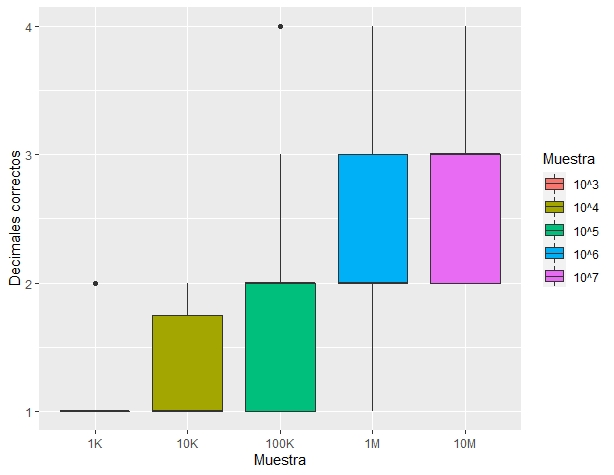
\includegraphics[width=150mm]{Figura2.jpeg} % archivo
    \caption{Cantidad de decimales que coinciden al variar el tamaño de la muestra en la comparación del valor $\pi$ calculado con el método Monte Carlo y el valor de $\pi$ considerado como $3.141592$.}
    \label{Figura2}
\end{figure}

Para analizar si existe una relación entre la variación del tamaño de muestra y la cantidad de decimales correctos, se realizó la prueba estadística \texttt{Kruskal Wallis} debido a que los resultados obtenidos no presentan normalidad. En el cuadro \ref{Cuadro4} se  resumen los resultados de la revisión de los supuestos para poder aplicar la prueba estadística. La normalidad por grupos se obtuvo con la prueba de \texttt{Shapiro Wilk}, y la homogeneidad de varianza se obtuvo con la prueba de \texttt{Levene}.

\begin{table}[ht]
\centering
\caption{Resultados del los supuestos para aplicar la prueba estadística.}
\smallskip

\begin{tabular}{ |p{5cm}|p{3.6cm}|}
 \hline
 Outliers & $10$ \\
 \hline
 Normalidad por grupo & $1\times 10^{3}$: $p$ = $1.78\times 10^{-10}$ $1\times 10^{4}$: $p$ = $2.09\times 10^{-8}$ $1\times 10^{5}$: $p$ = $1.32\times 10^{-4}$ $1\times 10^{6}$: $p$ = $1.54\times 10^{-3}$ $1\times 10^{7}$: $p$ = $3.11\times 10^{-6}$\\
 \hline
 Homogeneidad de varianza & $p$ = $1.12\times 10^{-5}$ \\
 \hline
\end{tabular}
\label{Cuadro4}
\end{table}

Al realizar la prueba \texttt{Kruskal Wallis} se obtienen los resultados mostrados en el cuadro \ref{Cuadro5}. 
\bigskip

\begin{table}[ht]
\centering
\caption{Resultados al aplicar la prueba estadística \texttt{Kruskal Wallis}.}
\smallskip

\begin{tabular}{ |p{2.1cm}|p{2.1cm}|}
 \hline
 Chi cuadrada & Valor de $p$ \\
 \hline
 $75.087$ & $1.91\times 10^{-15}$ \\
 \hline
\end{tabular}
\label{Cuadro5}
\end{table}

Hipótesis nula : Las medias son iguales en todos los grupos.
\smallskip

Hipótesis alternativa: Debido a que $p < 0.05$ se rechaza la hipótesis nula, es decir que si existen diferencias significativas entre las medias de los grupos. 
\bigskip

También se realizó la prueba de suma de rangos de \texttt{Wilcoxon} por pares, los resultados de esta prueba se resumen el cuadro \ref{Cuadro6}.

\newpage

\begin{table}[ht]
\centering
\caption{Resultados al aplicar la prueba \texttt{Wilcoxon}.}
\smallskip

\begin{tabular}{ |p{2.1cm}|p{2.1cm}|p{2.1cm}|p{2.1cm}|p{2.1cm}|}
 \hline
Valor de $p$ & $1\times 10^{3}$ & $1\times 10^{4}$ & $1\times 10^{5}$ & $1\times 10^{6}$\\
 \hline
 $1\times 10^{4}$ & $0.2006$ & - & - & - \\
 \hline
  $1\times 10^{5}$ & $5.6\times 10^{-4}$ & $0.0252$ & - & -\\
 \hline
  $1\times 10^{6}$ & $3.2\times 10^{-8}$ & $2.4\times 10^{-6}$ & $0.0478$ & - \\
 \hline
  $1\times 10^{7}$ & $9.7\times 10^{-11}$ & $4.1\times 10^{-9}$ & $0.0015$ & $0.2228$ \\
 \hline
\end{tabular}
\label{Cuadro6}
\end{table}

En los resultados mostrados en el cuadro \ref{Cuadro6} podemos ver que solamente las comparaciones de $1000$ con $10000$ y $1000000$ con $10000000$ tienen una $p > 0.05$, por lo tanto se puede determinar que solamente en estas comparaciones no existen diferencias significativas.
\bigskip

A continuación se muestra el código utilizado para realizar la prueba estadística \texttt{Kruskal Wallis}:

\lstset{style=mystyle}
\begin{lstlisting}[language=R, caption= Código para la prueba estadística \texttt{Kruskal Wallis} y la prueba \texttt{Wilcoxon}.]
#Estadisticas descriptivas
df %>%
  group_by(Muestra) %>%
  get_summary_stats(Decimales, type = "mean_sd")

#SUPUESTOS PARA ANOVA
#1:Outliers
df %>%
  group_by(Muestra) %>%
  identify_outliers(Decimales)

#2:Normalidad por Shapiro
df %>%
  group_by(Muestra) %>%
  shapiro_test(Decimales)

#3:Homogeneidad de varianza con prueba Levene
df %>%
  levene_test(Decimales~Muestra)

#PRUEBA ESTADISTICA KRUSKAL WALLIS
kruskal.test(Decimales ~ Muestra, data = df)

#PRUEBA WILCOXON
pairwise.wilcox.test(df$Decimales, df$Muestra)
\end{lstlisting}
\newpage
.
\bigskip

\section{Conclusi\'{o}n}
Con base en los diagramas caja-bigote y los resultados obtenidos en las pruebas estadísticas \texttt{Kruskal Wallis} puedo concluir que el hecho de variar el tamaño de la muestra si influye en la precisión de los resultados que se obtienen al evaluar funciones con el método Monte Carlo, también considero que si se utiliza un tamaño de muestra mayor a diez millones se tendría una mejor presición, esto lo intenté realizar pero debido a que la muestra es demasiado grande mi computadora se inhibió por varios minutos, por lo cual decidí no tomar muestras mayores a diez millones.
\smallskip

En general ésta práctica fue mucho de mi agrado porque la pude realizar sin grandes complicaciones como me sucedió en prácticas anteriores. 
\newpage
.
\bigskip

\bibliography{referencias}
\bibliographystyle{plainnat}

\end{document}